% Created 2013-02-26 mar 12:06
\documentclass{beamer}
\usepackage[utf8]{inputenc}
\usepackage[T1]{fontenc}
\usepackage{fixltx2e}
\usepackage{graphicx}
\usepackage{longtable}
\usepackage{float}
\usepackage{wrapfig}
\usepackage{soul}
\usepackage{textcomp}
\usepackage{marvosym}
\usepackage{wasysym}
\usepackage{latexsym}
\usepackage{amssymb}
\usepackage{hyperref}
\tolerance=1000
\usepackage{color}
\usepackage{listings}
\AtBeginSection[]{\begin{frame}<beamer>\frametitle{Contenidos}\tableofcontents[currentsection]\end{frame}}
\lstset{keywordstyle=\color{blue}, commentstyle=\color{gray!90}, basicstyle=\ttfamily\footnotesize, columns=fullflexible, breaklines=false,linewidth=\textwidth, backgroundcolor=\color{gray!23}, basewidth={0.5em,0.4em}, literate={á}{{\'a}}1 {ñ}{{\~n}}1 {é}{{\'e}}1 {ó}{{\'o}}1 {º}{{\textordmasculine}}1}
\usepackage{mathpazo}
\setbeamercovered{transparent}
\usefonttheme{serif} 
\usetheme{Goettingen}
\usepackage{fancyvrb}
\DefineVerbatimEnvironment{verbatim}{Verbatim}{fontsize=\tiny, formatcom = {\color{black!70}}}
\providecommand{\alert}[1]{\textbf{#1}}

\title{Estadística básica con R}
\author{Oscar Perpiñán Lamigueiro}
\date{\today}
\hypersetup{
  pdfkeywords={},
  pdfsubject={},
  pdfcreator={Emacs Org-mode version 7.8.11}}

\begin{document}

\maketitle




\section{Conjunto de datos}
\label{sec-1}
\begin{frame}
\frametitle{Conjunto de datos: swiss}
\label{sec-1-1}

Standardized fertility measure and socio-economic indicators for each
of 47 French-speaking provinces of Switzerland at about 1888. 6 variables in percent [0, 100]:

\begin{itemize}
\item Fertility:         Ig, ‘common standardizedfertility measure’
\item Agriculture:       \% of males involved in agriculture 
                               as occupation
\item Examination:       \% draftees receiving highest mark 
   on army examination
\item Education:         \% education beyond primary school for draftees.
\item Catholic:          \% ‘catholic’ (as opposed to ‘protestant’).
\item Infant.Mortality:  live births who live less than 1year.           
      
     All variables but ‘Fertility’ give proportions of the population.
\end{itemize}
\end{frame}
\begin{frame}[fragile]
\frametitle{Conjunto de datos: swiss}
\label{sec-1-2}



\lstset{language=R}
\begin{lstlisting}
data(swiss)

summary(swiss)
\end{lstlisting}


\begin{verbatim}
  Fertility      Agriculture     Examination      Education    
Min.   :35.00   Min.   : 1.20   Min.   : 3.00   Min.   : 1.00  
1st Qu.:64.70   1st Qu.:35.90   1st Qu.:12.00   1st Qu.: 6.00  
Median :70.40   Median :54.10   Median :16.00   Median : 8.00  
Mean   :70.14   Mean   :50.66   Mean   :16.49   Mean   :10.98  
3rd Qu.:78.45   3rd Qu.:67.65   3rd Qu.:22.00   3rd Qu.:12.00  
Max.   :92.50   Max.   :89.70   Max.   :37.00   Max.   :53.00  
   Catholic       Infant.Mortality
Min.   :  2.150   Min.   :10.80   
1st Qu.:  5.195   1st Qu.:18.15   
Median : 15.140   Median :20.00   
Mean   : 41.144   Mean   :19.94   
3rd Qu.: 93.125   3rd Qu.:21.70   
Max.   :100.000   Max.   :26.60
\end{verbatim}
\end{frame}
\begin{frame}[fragile]


\lstset{language=R}
\begin{lstlisting}
splom(swiss, pscale=0, type=c('p', 'smooth'),
      groups=swiss$Catholic > 50, xlab='')
\end{lstlisting}

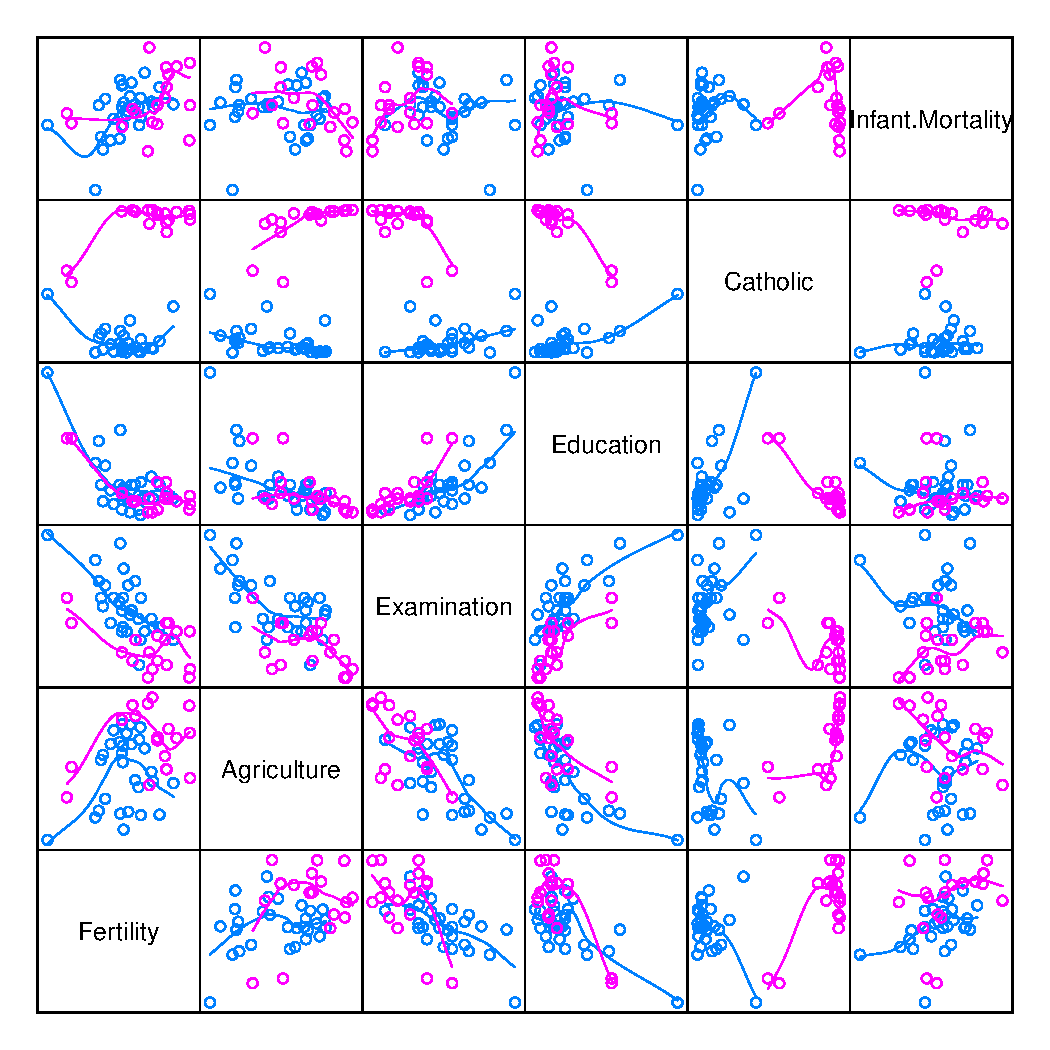
\includegraphics[width=.9\linewidth]{splomSwiss.pdf}
\end{frame}
\section{Estadística Univariante}
\label{sec-2}
\begin{frame}[fragile]
\frametitle{Resumir información}
\label{sec-2-1}


\lstset{language=R}
\begin{lstlisting}
summary(swiss)
\end{lstlisting}


\begin{verbatim}
  Fertility      Agriculture     Examination      Education    
Min.   :35.00   Min.   : 1.20   Min.   : 3.00   Min.   : 1.00  
1st Qu.:64.70   1st Qu.:35.90   1st Qu.:12.00   1st Qu.: 6.00  
Median :70.40   Median :54.10   Median :16.00   Median : 8.00  
Mean   :70.14   Mean   :50.66   Mean   :16.49   Mean   :10.98  
3rd Qu.:78.45   3rd Qu.:67.65   3rd Qu.:22.00   3rd Qu.:12.00  
Max.   :92.50   Max.   :89.70   Max.   :37.00   Max.   :53.00  
   Catholic       Infant.Mortality
Min.   :  2.150   Min.   :10.80   
1st Qu.:  5.195   1st Qu.:18.15   
Median : 15.140   Median :20.00   
Mean   : 41.144   Mean   :19.94   
3rd Qu.: 93.125   3rd Qu.:21.70   
Max.   :100.000   Max.   :26.60
\end{verbatim}


\lstset{language=R}
\begin{lstlisting}
mean(swiss$Fertility)
\end{lstlisting}

\begin{verbatim}
 [1] 70.14255
\end{verbatim}


\lstset{language=R}
\begin{lstlisting}
colMeans(swiss)
\end{lstlisting}

\begin{verbatim}
        Fertility      Agriculture      Examination        Education 
         70.14255         50.65957         16.48936         10.97872 
         Catholic Infant.Mortality 
         41.14383         19.94255
\end{verbatim}
\end{frame}
\begin{frame}[fragile]
\frametitle{Resumir información}
\label{sec-2-2}



\lstset{language=R}
\begin{lstlisting}
sd(swiss$Fertility)
\end{lstlisting}

\begin{verbatim}
 [1] 12.4917
\end{verbatim}


\lstset{language=R}
\begin{lstlisting}
sapply(swiss, sd)
\end{lstlisting}

\begin{verbatim}
        Fertility      Agriculture      Examination        Education 
        12.491697        22.711218         7.977883         9.615407 
         Catholic Infant.Mortality 
        41.704850         2.912697
\end{verbatim}
\end{frame}
\begin{frame}[fragile]
\frametitle{Generar datos aleatorios}
\label{sec-2-3}



\lstset{language=R}
\begin{lstlisting}
rnorm(10, mean=1, sd=.4)
\end{lstlisting}

\begin{verbatim}
  [1] 1.4773674 1.3867686 1.4616831 0.2660399 1.0762471 1.7757136 1.2287755
  [8] 0.9942296 0.9338062 1.2506691
\end{verbatim}


\lstset{language=R}
\begin{lstlisting}
runif(10, min=-3, max=3)
\end{lstlisting}

\begin{verbatim}
  [1] -0.4931618  0.2618546  1.1875716 -1.7761181 -2.5002714  2.2152122
  [7]  0.8830398  2.6895999 -0.9841917 -2.8621449
\end{verbatim}


\lstset{language=R}
\begin{lstlisting}
rweibull(n=10, shape=3, scale=2)
\end{lstlisting}

\begin{verbatim}
  [1] 1.1046997 1.4038783 2.1482313 2.1802392 2.4728738 1.6614008 1.5393820
  [8] 1.7977655 0.6410068 1.5485643
\end{verbatim}
\end{frame}
\begin{frame}[fragile]
\frametitle{Generar datos aleatorios}
\label{sec-2-4}



\lstset{language=R}
\begin{lstlisting}
x <- seq(1, 100, length=15)
x
\end{lstlisting}

\begin{verbatim}
  [1]   1.000000   8.071429  15.142857  22.214286  29.285714  36.357143
  [7]  43.428571  50.500000  57.571429  64.642857  71.714286  78.785714
 [13]  85.857143  92.928571 100.000000
\end{verbatim}


\lstset{language=R}
\begin{lstlisting}
sample(x)
\end{lstlisting}

\begin{verbatim}
  [1]  22.214286  85.857143   8.071429  71.714286   1.000000 100.000000
  [7]  29.285714  92.928571  50.500000  43.428571  64.642857  78.785714
 [13]  36.357143  57.571429  15.142857
\end{verbatim}


\lstset{language=R}
\begin{lstlisting}
sample(x, 5)
\end{lstlisting}

\begin{verbatim}
 [1] 15.142857  8.071429 36.357143 78.785714  1.000000
\end{verbatim}


\lstset{language=R}
\begin{lstlisting}
sample(x, 5, replace=TRUE)
\end{lstlisting}

\begin{verbatim}
 [1] 22.214286 85.857143 43.428571 85.857143  8.071429
\end{verbatim}
\end{frame}
\begin{frame}[fragile]
\frametitle{Tests}
\label{sec-2-5}



\lstset{language=R}
\begin{lstlisting}
t.test(swiss$Fertility, mu=70)
\end{lstlisting}


\begin{verbatim}

        One Sample t-test

data:  swiss$Fertility 
t = 0.0782, df = 46, p-value = 0.938
alternative hypothesis: true mean is not equal to 70 
95 percent confidence interval:
 66.47485 73.81025 
sample estimates:
mean of x 
 70.14255
\end{verbatim}


\lstset{language=R}
\begin{lstlisting}
wilcox.test(swiss$Fertility, mu=70)
\end{lstlisting}


\begin{verbatim}

        Wilcoxon signed rank test with continuity correction

data:  swiss$Fertility 
V = 592.5, p-value = 0.767
alternative hypothesis: true location is not equal to 70 

Mensajes de aviso perdidos
In wilcox.test.default(swiss$Fertility, mu = 70) :
  cannot compute exact p-value with ties
\end{verbatim}
\end{frame}
\begin{frame}[fragile]
\frametitle{Tests}
\label{sec-2-6}


\lstset{language=R}
\begin{lstlisting}
A <- rnorm(1000)
B <- rnorm(1000)
C <- rnorm(1000, sd=3)
\end{lstlisting}



\lstset{language=R}
\begin{lstlisting}
t.test(A, B)
\end{lstlisting}


\begin{verbatim}

        Welch Two Sample t-test

data:  A and B 
t = -0.856, df = 1995.848, p-value = 0.3921
alternative hypothesis: true difference in means is not equal to 0 
95 percent confidence interval:
 -0.12706615  0.04984534 
sample estimates:
   mean of x    mean of y 
-0.002826312  0.035784093
\end{verbatim}


\lstset{language=R}
\begin{lstlisting}
wilcox.test(A, B)
\end{lstlisting}

\begin{verbatim}
 
 	Wilcoxon rank sum test with continuity correction
 
 data:  A and B 
 W = 492610, p-value = 0.5672
 alternative hypothesis: true location shift is not equal to 0
\end{verbatim}
\end{frame}
\begin{frame}[fragile]
\frametitle{Tests}
\label{sec-2-7}


\lstset{language=R}
\begin{lstlisting}
t.test(A, C)
\end{lstlisting}


\begin{verbatim}

        Welch Two Sample t-test

data:  A and C 
t = -0.037, df = 1214.266, p-value = 0.9705
alternative hypothesis: true difference in means is not equal to 0 
95 percent confidence interval:
 -0.1999720  0.1925606 
sample estimates:
    mean of x     mean of y 
-0.0028263121  0.0008794018
\end{verbatim}


\lstset{language=R}
\begin{lstlisting}
wilcox.test(A, C)
\end{lstlisting}

\begin{verbatim}
 
 	Wilcoxon rank sum test with continuity correction
 
 data:  A and C 
 W = 509559, p-value = 0.4592
 alternative hypothesis: true location shift is not equal to 0
\end{verbatim}
\end{frame}
\begin{frame}[fragile]
\frametitle{Tests}
\label{sec-2-8}


\lstset{language=R}
\begin{lstlisting}
Religion <- ifelse(swiss$Catholic > 50,
                   'Catholic', 'Protestant')
\end{lstlisting}



\lstset{language=R}
\begin{lstlisting}
t.test(Fertility ~ Religion, data=swiss)
\end{lstlisting}


\begin{verbatim}

        Welch Two Sample t-test

data:  Fertility by Religion 
t = 2.7004, df = 26.742, p-value = 0.01186
alternative hypothesis: true difference in means is not equal to 0 
95 percent confidence interval:
  2.455904 18.024939 
sample estimates:
  mean in group Catholic mean in group Protestant 
                76.46111                 66.22069
\end{verbatim}


\lstset{language=R}
\begin{lstlisting}
wilcox.test(Fertility ~ Religion, data=swiss)
\end{lstlisting}


\begin{verbatim}

        Wilcoxon rank sum test with continuity correction

data:  Fertility by Religion 
W = 409.5, p-value = 0.0012
alternative hypothesis: true location shift is not equal to 0 

Mensajes de aviso perdidos
In wilcox.test.default(x = c(83.1, 92.5, 76.1, 83.8, 92.4, 82.4,  :
  cannot compute exact p-value with ties
\end{verbatim}
\end{frame}
\section{Regresión lineal}
\label{sec-3}
\begin{frame}[fragile]
\frametitle{Fertilidad y educación}
\label{sec-3-1}


\lstset{language=R}
\begin{lstlisting}
lmFertEdu <- lm(Fertility ~ Education,
                data = swiss)
summary(lmFertEdu)
\end{lstlisting}


\begin{verbatim}

Call:
lm(formula = Fertility ~ Education, data = swiss)

Residuals:
    Min      1Q  Median      3Q     Max 
-17.036  -6.711  -1.011   9.526  19.689 

Coefficients:
            Estimate Std. Error t value Pr(>|t|)    
(Intercept)  79.6101     2.1041  37.836  < 2e-16 ***
Education    -0.8624     0.1448  -5.954 3.66e-07 ***
---
Signif. codes:  0 ‘***’ 0.001 ‘**’ 0.01 ‘*’ 0.05 ‘.’ 0.1 ‘ ’ 1 

Residual standard error: 9.446 on 45 degrees of freedom
Multiple R-squared: 0.4406,     Adjusted R-squared: 0.4282 
F-statistic: 35.45 on 1 and 45 DF,  p-value: 3.659e-07
\end{verbatim}
\end{frame}
\begin{frame}[fragile]
\frametitle{Fertilidad y educación}
\label{sec-3-2}


\lstset{language=R}
\begin{lstlisting}
coef(lmFertEdu)
\end{lstlisting}

\begin{verbatim}
 (Intercept)   Education 
  79.6100585  -0.8623503
\end{verbatim}


\lstset{language=R}
\begin{lstlisting}
residuals(lmFertEdu)
\end{lstlisting}


\begin{verbatim}
Courtelary     Delemont Franches-Mnt      Moutier   Neuveville   Porrentruy 
10.9381450   11.2510941   17.2016929   12.2263935   10.2251959    2.5263935 
     Broye        Glane      Gruyere       Sarine      Veveyse        Aigle 
10.2263935   19.6887438    8.8263935   14.5004953   12.6640432   -5.1618550 
   Aubonne     Avenches     Cossonay    Echallens     Grandson     Lausanne 
-6.6736065   -0.3618550  -13.5983071   -9.5853579   -1.0112562    0.2357497 
 La Vallee       Lavaux       Morges       Moudon        Nyone         Orbe 
-8.0630527   -6.7489059   -5.4865556  -12.0230077  -12.6618550  -17.0359568 
      Oron      Payerne Paysd'enhaut        Rolle        Vevey      Yverdon 
-6.2477082    1.4887438   -5.0230077  -10.4865556   -4.9254030   -7.3112562 
   Conthey    Entremont       Herens     Martigwy      Monthey   St Maurice 
-2.3853579   -5.1359568   -0.5853579   -3.9359568    2.3769923   -6.8489059 
    Sierre         Sion       Boudry La Chauxdfnd     Le Locle    Neuchatel 
15.1769923   10.9004953    1.1381450   -4.4242053    4.3004953   12.3851508 
Val de Ruz ValdeTravers V. De Geneve  Rive Droite  Rive Gauche 
 4.0263935   -5.9736065    1.0945070   -9.9019000  -11.8019000
\end{verbatim}


\lstset{language=R}
\begin{lstlisting}
fitted.values(lmFertEdu)
\end{lstlisting}


\begin{verbatim}
Courtelary     Delemont Franches-Mnt      Moutier   Neuveville   Porrentruy 
  69.26186     71.84891     75.29831     73.57361     66.67480     73.57361 
     Broye        Glane      Gruyere       Sarine      Veveyse        Aigle 
  73.57361     72.71126     73.57361     68.39950     74.43596     69.26186 
   Aubonne     Avenches     Cossonay    Echallens     Grandson     Lausanne 
  73.57361     69.26186     75.29831     77.88536     72.71126     55.46425 
 La Vallee       Lavaux       Morges       Moudon        Nyone         Orbe 
  62.36305     71.84891     70.98656     77.02301     69.26186     74.43596 
      Oron      Payerne Paysd'enhaut        Rolle        Vevey      Yverdon 
  78.74771     72.71126     77.02301     70.98656     63.22540     72.71126 
   Conthey    Entremont       Herens     Martigwy      Monthey   St Maurice 
  77.88536     74.43596     77.88536     74.43596     77.02301     71.84891 
    Sierre         Sion       Boudry La Chauxdfnd     Le Locle    Neuchatel 
  77.02301     68.39950     69.26186     70.12421     68.39950     52.01485 
Val de Ruz ValdeTravers V. De Geneve  Rive Droite  Rive Gauche 
  73.57361     73.57361     33.90549     54.60190     54.60190
\end{verbatim}
\end{frame}
\begin{frame}[fragile]
\frametitle{Fertilidad, educación y religión}
\label{sec-3-3}


\lstset{language=R}
\begin{lstlisting}
lmFertEduCat <- lm(Fertility ~ Education + Catholic,
                   data = swiss)
summary(lmFertEduCat)
\end{lstlisting}


\begin{verbatim}

Call:
lm(formula = Fertility ~ Education + Catholic, data = swiss)

Residuals:
    Min      1Q  Median      3Q     Max 
-15.042  -6.578  -1.431   6.122  14.322 

Coefficients:
            Estimate Std. Error t value Pr(>|t|)    
(Intercept) 74.23369    2.35197  31.562  < 2e-16 ***
Education   -0.78833    0.12929  -6.097 2.43e-07 ***
Catholic     0.11092    0.02981   3.721  0.00056 ***
---
Signif. codes:  0 ‘***’ 0.001 ‘**’ 0.01 ‘*’ 0.05 ‘.’ 0.1 ‘ ’ 1 

Residual standard error: 8.331 on 44 degrees of freedom
Multiple R-squared: 0.5745,     Adjusted R-squared: 0.5552 
F-statistic:  29.7 on 2 and 44 DF,  p-value: 6.849e-09
\end{verbatim}
\end{frame}
\begin{frame}[fragile]
\frametitle{Lo mismo con \texttt{update}}
\label{sec-3-4}


\lstset{language=R}
\begin{lstlisting}
lmFertEduCat <- update(lmFertEdu, . ~ . + Catholic,
                       data = swiss)
summary(lmFertEduCat)
\end{lstlisting}


\begin{verbatim}

Call:
lm(formula = Fertility ~ Education + Catholic, data = swiss)

Residuals:
    Min      1Q  Median      3Q     Max 
-15.042  -6.578  -1.431   6.122  14.322 

Coefficients:
            Estimate Std. Error t value Pr(>|t|)    
(Intercept) 74.23369    2.35197  31.562  < 2e-16 ***
Education   -0.78833    0.12929  -6.097 2.43e-07 ***
Catholic     0.11092    0.02981   3.721  0.00056 ***
---
Signif. codes:  0 ‘***’ 0.001 ‘**’ 0.01 ‘*’ 0.05 ‘.’ 0.1 ‘ ’ 1 

Residual standard error: 8.331 on 44 degrees of freedom
Multiple R-squared: 0.5745,     Adjusted R-squared: 0.5552 
F-statistic:  29.7 on 2 and 44 DF,  p-value: 6.849e-09
\end{verbatim}
\end{frame}
\begin{frame}[fragile]
\frametitle{Fertilidad, educación, religión y agricultura}
\label{sec-3-5}


\lstset{language=R}
\begin{lstlisting}
lmFertEduCatAgr <- lm(Fertility ~ Education + Catholic + Agriculture,
                      data = swiss)
summary(lmFertEduCatAgr)
\end{lstlisting}


\begin{verbatim}

Call:
lm(formula = Fertility ~ Education + Catholic + Agriculture, 
    data = swiss)

Residuals:
    Min      1Q  Median      3Q     Max 
-15.178  -6.548   1.379   5.822  14.840 

Coefficients:
            Estimate Std. Error t value Pr(>|t|)    
(Intercept) 86.22502    4.73472  18.211  < 2e-16 ***
Education   -1.07215    0.15580  -6.881 1.91e-08 ***
Catholic     0.14520    0.03015   4.817 1.84e-05 ***
Agriculture -0.20304    0.07115  -2.854  0.00662 ** 
---
Signif. codes:  0 ‘***’ 0.001 ‘**’ 0.01 ‘*’ 0.05 ‘.’ 0.1 ‘ ’ 1 

Residual standard error: 7.728 on 43 degrees of freedom
Multiple R-squared: 0.6423,     Adjusted R-squared: 0.6173 
F-statistic: 25.73 on 3 and 43 DF,  p-value: 1.089e-09
\end{verbatim}
\end{frame}
\begin{frame}[fragile]
\frametitle{Lo mismo con \texttt{update}}
\label{sec-3-6}


\lstset{language=R}
\begin{lstlisting}
lmFertEduCatAgr <- update(lmFertEduCat, . ~ . + Agriculture,
                          data = swiss)
summary(lmFertEduCatAgr)
\end{lstlisting}


\begin{verbatim}

Call:
lm(formula = Fertility ~ Education + Catholic + Agriculture, 
    data = swiss)

Residuals:
    Min      1Q  Median      3Q     Max 
-15.178  -6.548   1.379   5.822  14.840 

Coefficients:
            Estimate Std. Error t value Pr(>|t|)    
(Intercept) 86.22502    4.73472  18.211  < 2e-16 ***
Education   -1.07215    0.15580  -6.881 1.91e-08 ***
Catholic     0.14520    0.03015   4.817 1.84e-05 ***
Agriculture -0.20304    0.07115  -2.854  0.00662 ** 
---
Signif. codes:  0 ‘***’ 0.001 ‘**’ 0.01 ‘*’ 0.05 ‘.’ 0.1 ‘ ’ 1 

Residual standard error: 7.728 on 43 degrees of freedom
Multiple R-squared: 0.6423,     Adjusted R-squared: 0.6173 
F-statistic: 25.73 on 3 and 43 DF,  p-value: 1.089e-09
\end{verbatim}
\end{frame}
\begin{frame}[fragile]
\frametitle{Lo mismo con \texttt{update}}
\label{sec-3-7}


\lstset{language=R}
\begin{lstlisting}
lmFertEduCatAgr <- update(lmFertEdu, . ~ . + Catholic + Agriculture,
                          data = swiss)
summary(lmFertEduCatAgr)
\end{lstlisting}


\begin{verbatim}

Call:
lm(formula = Fertility ~ Education + Catholic + Agriculture, 
    data = swiss)

Residuals:
    Min      1Q  Median      3Q     Max 
-15.178  -6.548   1.379   5.822  14.840 

Coefficients:
            Estimate Std. Error t value Pr(>|t|)    
(Intercept) 86.22502    4.73472  18.211  < 2e-16 ***
Education   -1.07215    0.15580  -6.881 1.91e-08 ***
Catholic     0.14520    0.03015   4.817 1.84e-05 ***
Agriculture -0.20304    0.07115  -2.854  0.00662 ** 
---
Signif. codes:  0 ‘***’ 0.001 ‘**’ 0.01 ‘*’ 0.05 ‘.’ 0.1 ‘ ’ 1 

Residual standard error: 7.728 on 43 degrees of freedom
Multiple R-squared: 0.6423,     Adjusted R-squared: 0.6173 
F-statistic: 25.73 on 3 and 43 DF,  p-value: 1.089e-09
\end{verbatim}
\end{frame}
\begin{frame}[fragile]
\frametitle{anova}
\label{sec-3-8}


\lstset{language=R}
\begin{lstlisting}
anova(lmFertEdu, lmFertEduCat, lmFertEduCatAgr)
\end{lstlisting}


\begin{verbatim}
Analysis of Variance Table

Model 1: Fertility ~ Education
Model 2: Fertility ~ Education + Catholic
Model 3: Fertility ~ Education + Catholic + Agriculture
  Res.Df    RSS Df Sum of Sq      F    Pr(>F)    
1     45 4015.2                                  
2     44 3054.2  1    961.07 16.093 0.0002365 ***
3     43 2567.9  1    486.28  8.143 0.0066235 ** 
---
Signif. codes:  0 ‘***’ 0.001 ‘**’ 0.01 ‘*’ 0.05 ‘.’ 0.1 ‘ ’ 1
\end{verbatim}
\end{frame}
\begin{frame}[fragile]
\frametitle{Fertilidad contra todo}
\label{sec-3-9}


\lstset{language=R}
\begin{lstlisting}
lmFert <- lm(Fertility ~ ., data=swiss)

summary(lmFert)
\end{lstlisting}


\begin{verbatim}

Call:
lm(formula = Fertility ~ ., data = swiss)

Residuals:
     Min       1Q   Median       3Q      Max 
-15.2743  -5.2617   0.5032   4.1198  15.3213 

Coefficients:
                 Estimate Std. Error t value Pr(>|t|)    
(Intercept)      66.91518   10.70604   6.250 1.91e-07 ***
Agriculture      -0.17211    0.07030  -2.448  0.01873 *  
Examination      -0.25801    0.25388  -1.016  0.31546    
Education        -0.87094    0.18303  -4.758 2.43e-05 ***
Catholic          0.10412    0.03526   2.953  0.00519 ** 
Infant.Mortality  1.07705    0.38172   2.822  0.00734 ** 
---
Signif. codes:  0 ‘***’ 0.001 ‘**’ 0.01 ‘*’ 0.05 ‘.’ 0.1 ‘ ’ 1 

Residual standard error: 7.165 on 41 degrees of freedom
Multiple R-squared: 0.7067,     Adjusted R-squared: 0.671 
F-statistic: 19.76 on 5 and 41 DF,  p-value: 5.594e-10
\end{verbatim}
\end{frame}
\begin{frame}[fragile]
\frametitle{Elegir un modelo}
\label{sec-3-10}


\lstset{language=R}
\begin{lstlisting}
anova(lmFert)
\end{lstlisting}


\begin{verbatim}
Analysis of Variance Table

Response: Fertility
                 Df  Sum Sq Mean Sq F value    Pr(>F)    
Agriculture       1  894.84  894.84 17.4288 0.0001515 ***
Examination       1 2210.38 2210.38 43.0516 6.885e-08 ***
Education         1  891.81  891.81 17.3699 0.0001549 ***
Catholic          1  667.13  667.13 12.9937 0.0008387 ***
Infant.Mortality  1  408.75  408.75  7.9612 0.0073357 ** 
Residuals        41 2105.04   51.34                      
---
Signif. codes:  0 ‘***’ 0.001 ‘**’ 0.01 ‘*’ 0.05 ‘.’ 0.1 ‘ ’ 1
\end{verbatim}
\end{frame}
\begin{frame}[fragile]
\frametitle{Elegir un modelo}
\label{sec-3-11}


\lstset{language=R}
\begin{lstlisting}
stepFert <- step(lmFert)
summary(stepFert)
\end{lstlisting}


\begin{verbatim}
Start:  AIC=190.69
Fertility ~ Agriculture + Examination + Education + Catholic + 
    Infant.Mortality

                   Df Sum of Sq    RSS    AIC
- Examination       1     53.03 2158.1 189.86
<none>                          2105.0 190.69
- Agriculture       1    307.72 2412.8 195.10
- Infant.Mortality  1    408.75 2513.8 197.03
- Catholic          1    447.71 2552.8 197.75
- Education         1   1162.56 3267.6 209.36

Step:  AIC=189.86
Fertility ~ Agriculture + Education + Catholic + Infant.Mortality

                   Df Sum of Sq    RSS    AIC
<none>                          2158.1 189.86
- Agriculture       1    264.18 2422.2 193.29
- Infant.Mortality  1    409.81 2567.9 196.03
- Catholic          1    956.57 3114.6 205.10
- Education         1   2249.97 4408.0 221.43

Call:
lm(formula = Fertility ~ Agriculture + Education + Catholic + 
    Infant.Mortality, data = swiss)

Residuals:
     Min       1Q   Median       3Q      Max 
-14.6765  -6.0522   0.7514   3.1664  16.1422 

Coefficients:
                 Estimate Std. Error t value Pr(>|t|)    
(Intercept)      62.10131    9.60489   6.466 8.49e-08 ***
Agriculture      -0.15462    0.06819  -2.267  0.02857 *  
Education        -0.98026    0.14814  -6.617 5.14e-08 ***
Catholic          0.12467    0.02889   4.315 9.50e-05 ***
Infant.Mortality  1.07844    0.38187   2.824  0.00722 ** 
---
Signif. codes:  0 ‘***’ 0.001 ‘**’ 0.01 ‘*’ 0.05 ‘.’ 0.1 ‘ ’ 1 

Residual standard error: 7.168 on 42 degrees of freedom
Multiple R-squared: 0.6993,     Adjusted R-squared: 0.6707 
F-statistic: 24.42 on 4 and 42 DF,  p-value: 1.717e-10
\end{verbatim}
\end{frame}
\begin{frame}[fragile]
\frametitle{Elegir un modelo}
\label{sec-3-12}


\lstset{language=R}
\begin{lstlisting}
stepFert$anova
\end{lstlisting}

\begin{verbatim}
            Step Df Deviance Resid. Df Resid. Dev      AIC
 1               NA       NA        41   2105.043 190.6913
 2 - Examination  1 53.02656        42   2158.069 189.8606
\end{verbatim}
\end{frame}

\end{document}